\documentclass[12pt]{article}

\usepackage{pset}
\usepackage{math}
\usepackage{util}
\usepackage{ufont}

\usepackage[normalem]{ulem}
\newcommand*{\X}{\mathfrak{X}}
\newcommand*{\Mod}{\mathcal{M}}
\newcommand*{\ms}{\mathcal{M}}
\newcommand*{\ps}{\mathcal{P}\,}


\title{Thesis Journal}
\author{Aaron Pribadi}
\date{}

\begin{document}

\maketitle

\section{September 9, 2011}

\subsection{Introduction}

I would like to work on a problem in algebraic statistics, and more specifically
a problem about graphical models.  I do not yet have a coherent `story' for the
background of a problem, so I will instead discuss some topics in a close
neighborhood of what I want to work on.


\subsection{Graphical models}

Independence conditions arise naturally in many probabilistic models.  A
graphical model is a probabilistic model for which a graph (directed or
undirected) represents the conditional independence structure between random
variables. 

Let $G$ be a graph with vertex set $V$.  Suppose that $(X_\alpha)_{\alpha \in
V}$ are random variables taking values in probability spaces
$(\X_\alpha)_{\alpha \in V}$.  Usually the $X_\alpha$ are either discrete or
real-valued.  The joint probability of $X = (X_\alpha)$ is said to
factor with respect to $G$ if the probability density is
\[
    P[X_1, \ldots, X_n] = 
        \prod_\alpha P[X_\alpha \mid X_\beta, \beta \text{ is a parent of }
        \alpha]
\]
that is, the dependence of a random variable on the other variables is
completely captured by its dependence on its immediate parents (i.e. on the
variables having directed edges into it).  We can also formulate an equivalent
statement in terms of conditional independence statements.

In the case of an undirected graph, it is known (the Hammersley–Clifford
theorem) that the probability density factors as
\[
    P[X_1, \ldots, X_n] = 
        \prod_{S \in C(G)} P[X_\alpha \mid X_\beta, \beta \in S]
\]
where the $S$ are complete subgraphs (cliques) of $G$.

Graphical models turn up in a number of places -- some include Bayesian networks
(directed) and Markov random fields (undirected) in statistics, Boltzmann
machines in machine learning, and Ising models (particle spins in a lattice) in
statistical mechanics.

\subsection{Boltzmann machines}

A Boltzmann machine factors with respect to an undirected graph, and in addition
assumes that the variables only have pairwise interactions.

Concretely, let the random variable $X = (X_i)_{1 \le i \le n}$ take values in
$\{0,1\}^n$, and let $\theta = (\theta_{ij})$ be a symmetric $n \times n$
matrix.  Then $\theta$ parametrizes a family of probability distributions.

We can regard 
\[
    H_\theta(X) = \sum_{i < j} \theta_{ij} X_i X_j + \sum_i \theta_i X_i
\]
as the energy of the system.  Then the probability of $X$ is
\[
    P_\theta[X] = \frac{\exp(- H_\theta(X))}{Z_\theta}
\]
where $Z_\theta$ is the normalizing factor
\[
    Z_\theta = \sum_{X \in \{0,1\}^n} \exp(-H_\theta(X))))
\]
known as the partition function.

Notice that the `exponent of sum' form of the probability density directly
corresponds to a `product of terms' form, from which we can derive conditional
independence statements if some of the entries $\theta_{ij}$ are zero.

The Boltzmann machine is inspired by ideas statistical mechanics, where the
distribution is known as the Ising model.  Also, restricted Boltzmann machines
(RBMs) have recently become a building block for an important technique in
machine learning -- deep belief networks.

A RBM has some number of `observed' variables $X_1, \ldots, X_m$ and hidden
variables $X_{m+1}, \ldots, X_n$.  The graph for the RBM is the complete
bipartite graph, where every edge is between an observed and hidden variable,
i.e. $\theta_{ij} = 0$ if $i,j \le m$ or $i,j \ge m+1$.

Because the hidden variables are not observed, in order to fit the model's
parameters to the data we consider the marginalized probabilities
\[
    P_\theta[X_1, \ldots, X_m] = \sum_{(X_{m+1}, \ldots, X_n) \in \{0,1\}^{n-m}}
        P_\theta[X_1, \ldots, X_n].
\]
With a fitted parameter $\theta$ and an observed value $X_1, \ldots, X_m$, we can
also compute a probability distribution over the hidden variables; in some
sense, the hidden variables constitute an `explanation' for the data.


\subsection{The (algebraic) geometry of probability models}

A probability distribution over a finite set of size $n$ corresponds with a
point in the \emph{probability simplex}
\[
    \Delta_{n-1} = 
    \left\{(x_1, \ldots, x_{n}) \mid \sum_{i=1}^n x_i= 1, x_i \ge 0 \right\} 
    \cong 
    \left\{(x_1, \ldots, x_n) \mid \sum_{i=1}^{n-1} x_i \le 1, x_i \ge 0 \right\}
\]
of dimension $n-1$.  We can think of a probability model as a subspace 
$\Mod \subset \Delta_{n-1}$.

One way to select a particular probability distribution $p$ from a model $\Mod$
is by \emph{maximum likelihood}.  That is, given observations $X^{(1)}, \ldots,
X^{(N)}$ we attempt to maximize
\[
    L(p \mid X^{(1)}, \ldots, X^{(N)}) = \prod_{i=1}^N p(X^{(i)}
\]
though in practice the negative log-likelihood $l(p, X^{(i)}) = -\log L(p, X^{(i)}$ is
often used (this is a `loss' function, and the losses of the observations are
summed).

From the viewpoint of algebraic geometry, we will usually stipulate that models
are semialgebraic sets, that is, subsets of $\R^n$ that are determined by
polynomial equations and polynomial inequalities.  Real algebraic geometry
(which studies these objects) can be difficult, so sometimes the field is
extended to the complex numbers and/or the Zariski closure of the set is
considered.

Oftentimes, to compute things we will want some rational parametrization $\R^n
\supset U \to \Mod$ of the model.

Using the computational tools available to algebraic geometry (and with problem
sizes, e.g. dimension, that are extremely small) it is sometimes possible to
answer questions like `what is the maximum likelihood parameter' exactly.

The overall hope of approaches like this is (from what I can see) to apply the
tools of geometry to the problems of statistics.  (Compare with `information
geometry', the application of the techniques of differential (esp. Riemannian)
geometry to problems in probability theory, pioneered in the 1980s -- I don't
know how much it has caught on.)  One potential gain from this approach is that
`coordinate-invariance' comes more naturally than usual.


\subsection{Machine learning (and deep learning)}

Machine learning involves algorithmically taking data in order to perform better
at some task.  Abstractly, its goal is similar to that of statistics -- to learn
from data.  The emphasis, however, tends to be toward large data sets, efficient
algorithms (for those large data sets), and fewer assumptions on models
(`non-parametric' statistics).  

Machine learning is studied both by computer scientists and statisticians (who
sometimes call it statistical learning).  (A very good introduction, and one
from which I have taken much of my viewpoint on ML, is \textit{The Elements of
Statistical Learning} by Hastie, Tibshirani, and Friedman -- three
statisticians.)

One very common task is the classification problem.  Here, observations are
points in some (complicated, high-dimensional) space $X$, and the goal is to
assign an observation $x \in X$ to a class label from some finite set $\{A, B,
\ldots \}$.  It can be viewed as a problem where we are attempting to
approximate a function $f : X \to \{A, B, \ldots\}$ given a number of observed
class labels $f(x^{(i)})$.  Of course, this problem is impossible without some very
strong constraints on the type of function (the `model').  You can transform the
classification problem into a problem of estimating a probability distribution
by simply considering the joint distribution over observations and labels.

Most successful algorithms are in some sense `only a step or two away from
linear'.  A basic approach (to, say, binary classification) is to try to
separate the points in the two classes by some hyperplane.  A modification (used
by support vector machines (SVMs)) is to transform the data to some even-higher
dimensional space (infinite, perhaps), and to separate by a hyperplane there.
Another common approach is to have some family of basis functions, and to
consider linear combinations of them.

However, for some problems these techniques may not be enough.  This has
prompted (with some success only in the last ten years?) the creation of
so-called `deep learning' methods, which have `many layers of non-linearity'.
One very important method (perhaps the \emph{most important} so far) is called
the deep belief network and involves stacking restricted Boltzmann machines and
training them greedily.  (Professor Keller, I think, has done some work with
deep belief networks.)  

Deep belief networks can be, however, extremely difficult to optimize.
Monte-Carlo-Markov-Chain (MCMC) techniques are necessary, and esoteric sounding
things like `importance sampling' and `simulated annealing' are used to improve
performance.  (The general subject area is called `stochastic optimization', I
think.  Remember that we do not need exactly optimal solutions, but only
solutions that are `good enough'.)

These and similar methods have performed well on some problems.  One `standard'
example that shows up a lot in papers is the MNIST dataset of handwritten
digits.  In some cases, these algorithms solve an even harder problem than what
humans do -- the `permutation invariant' problem delivers the pixels of the
image as a vector with no a priori knowledge of the geometry of the image.

\subsection{Prior work}

For the algebraic geometry of graphical models, one paper is `On the toric
algebra of graphical models' (Geiger, Meek, Sturmfels -- 2006).  A book-length
account that covers graphical models, among other topics in algebraic
statistics, is `Lectures on Algebraic Statistics' (Drton, Sturmfels, Sullivant
-- 2009).  

Papers that have focused on specific types of graphical models include
`Algebraic Geometry of Bayesian Networks' (Garcia, Stillman, Sturmfels -- 2003)
and `Geometry of the restricted Boltzmann Machine' (Cueto, Morton, and Sturmfels
-- 2009).  

Inspired by questions in phylogenetics, tropical geometry has been applied to
questions in algebraic statistics (incl. graphical models).  See the paper
`Tropical Geometry of Statistical Models' (Pachter, Sturmfels -- 2003) and the
book `Algebraic Statistics for Computational Biology' (Pachter, Sturmfels --
2005).

Another book, which builds theory for considering optimization problems from the
viewpoint of algebraic statistics is `Algebraic Geometry and Statistical
Learning Theory' (Watanabe 2009).

From the machine learning side, questions in deep learning have spawned a large
number of papers, but an early and important one is `A fast learning algorithm for
deep belief nets' (Hinton 2007).  A good survey paper on the need for and
approaches to deep learning is `Learning deep architectures for AI' (Bengio
2009).

One very recent type of graphical model that encompasses models with tractable
partition functions was introduced in `Sum-Product Networks: A New Deep
Architecture' (Domingos, Poon 2011).

\subsection{Where to go from here}

One possibility for a problem to work on is to simply extend Sturmfels' work on
the restricted Boltzmann machine.  There is some distance yet between examining
its geometry and having something useful to say about the optimization problem.

\section{September 16, 2011}


\subsection{The restricted Boltzmann machine}

We describe a restricted Boltzmann machine (RBM); some of this is a repeat from
earlier.

An RBM with $n$ visible variables and $k$ hidden variables is a model with
states $(v, h)$ where $v \in \{0,1\}^n$ and $h \in \{0,1\}^k$.  It is
parametrized by a real $k \times n$ matrix and real vectors $b \in \R^n$, $c \in
\R^k$ (so it has a total of $nk + n + k$ parameters).  The unnormalized joint
distribution is
\[
    \psi(v, h) = \exp(h^T W v + b^Tv + c^T h).
\]
The probability distribution over the visible variables is 
\[
    p(v) = \frac 1 Z \cdot \sum_{h \in \{0,1\}^k} \psi(v, h)
\]
where $Z = \sum_{v,h} \psi(v, h)$ is the \emph{partition function}.  (This
procedure, of defining a joint probability distribution and then
\emph{marginalizing} over hidden variables, is a common one.)

Because the only interactions between variables are pairwise between one visible
and one hidden, the model factors according to the complete bipartite graph
$K_{n,k}$.  (Notice that the terms in the sum inside the $\exp$ become
multiplicative factors.  Thus terms that only involve some subset of variables
correspond to multiplicative factors that only involve those variables --- from
which we can derive the appropriate independence conditions.)

\subsection{Summary of `Geometry of the restricted Boltzmann machine'}

Now to the paper.  In order to move to an algebro-geometric presentation, the
paper uses the parametrization
\[
    \gamma_i = \exp(c_i)
    \qquad
    \omega_{ij} = \exp(W_{ij})
    \qquad
    \beta_j = \exp(b_j)
\]
with which
\[
    \psi(v, h) = \prod_{i=1}^k \gamma_i^{h_i}
        \cdot 
        \prod_{i=1}^k \prod_{j=1}^n \omega_{ij}^{h_i v_j}
        \cdot
        \prod_{j=1}^n \beta_j^{v_j}.
\]
The above is a monomial, and is not actually very scary.  The partition $Z$ is
also polynomial in the parameters, so the map $\R^{nk+n+k} \to
\Delta_{2^n-1}$ from parameters to probability distributions given by $p(v)$ is
then a rational map.  The image $M_n^k \subset \Delta_{2^n - 1}$ of the map is a
semialgebraic set.

The author considers both the semialgebraic set $M_n^k \subset \Delta_{2^n - 1}$
and the variety $V_n^k$ which is the Zariski closure of $M_n^k$ in complex
projective space.  Some results and conjectures on dimension are given.

In the absence of `problems', one would expect that $M_n^k$ has the same
dimension as its preimage $\R^{nk + n + k}$.  The dimension of $M_n^k$ of course
cannot exceed the dimension of its containing space, $2^n - 1$.  Thus the author
conjectures that
\[
    \dim M_n^k = \min\{nk+n+k, 2^n -1\}
\]
in $\Delta_{2^n-1}$, and proves the conjecture for most usual values of $n,k$,
i.e. for $k \le 2^{n - \lceil \log_2(n+1) \rceil}$.

The author also shows that the varieties $M_n^k$ and $V_n^k$ `factor'.
Specifically, they factor as \emph{Hadamard powers}
\[
    V_n^k = (V_n^1)^{[k]}
    \qquad
    M_n^k = (M_n^1)^{[k]}.
\]
Then $M_n^1$ and $V_n^1$ are examined.  One result proved is that $V_n^1$
conincides with the first secant variety of the \emph{Segre embedding} of the
product of projective lines $(\Proj^1)^n$ into $\Proj^{2^n-1}$.  Also, $M_n^1$
can be seen as a \emph{mixture model} of two independence models and has a
`star-shaped' independence graph.

(Both the Hadamard product and the Segre embedding are fairly standard
constructions.)

Another way to look at an RBM (and, indeed, the reason that it is useful for
deep belief networks) is as an `inference function'.  You give it an observed
value for the visible nodes, and you get a conditional probability distribution
over the hidden nodes $p(h \mid v)$.  The value $h \in \{0,1\}^k$ of maximal
likelihood is an `explanation' of the observed datum.

It turns out that the components $h_i$ of $h$ are, viewed as functions of $v$,
`linear threshold functions'.  Basically, the values of $v$ are vertices of a
hypercube, and the decision boundary of whether $h_i = 0$ or $1$ is a hyperplane
through the hypercube.

The author also examines the RBM using tropical geometry, but I am not familiar
enough with it to give a good explanation.

\subsection{Summary of Montufar}

I haven't written this up yet

\subsection{Questions}

How does tropical geometry fit into the picture?  The paper \cite{PS03} may help.

Can any of these results (incl. tropical) help with the training being done with
DBNs, i.e. with stochastic optimization on networks with a large number of
nodes?

As far as where to go with this, one direction is simply to `stack up' the RBMs:
what is the (algebraic) geometry of the deep belief network?  It also looks like
the mixture model perspective helps to understand the RBM -- can in also, from
the alg-geo point of view, help with the DBN?

The variety $\Proj^1 \times \cdots \times \Proj^1$ appears to play an important
role with the RBM \dots.

Another thing to look at:  It appears that the bounds on the number of hidden
units for universal approximators require a model with \emph{much much} more
parameters than are required to solely match the dimension requirements.  When
the RBM/DBN is at full dimension but does not cover the whole range of possible
distributions, what do the `holes' look like?

\section{September 23, 2011}

Short (10 min) presentation to thesis group was last Tuesday.

\subsection{Thoughts on an expository paper}

The presentation I did on Tuesday (with \sout{a few} many expanded topics) could
be one good ordering with which to approach the topic somewhat pedagogically.
That is, the order
\begin{itemize}
\item Brief introduction to algebraic statistics and algebraic geometry (what
are they?)
\item The probability simplex (making probability geometric)
\item Example: the independence model
\item Example: mixture models and hidden values
\item Statistical learning -- models, maximum likelihood, and model selection
criteria
\item Statistical learning -- common optimization algorithms (?? optional ??)
\item The RBM (restricted Boltzmann machine) -- definition
\item The RBM -- marginalization and the interpretation as an inference function
\item The RBM -- its algebraic geometry
\item Graphical models -- a taxonomy, applications (?? optional ??)
\item Graphical models -- computational concerns, and algebraic techniques (?? optional ??)
\item Machine learning -- goals, techniques, and trends (`deep learning')
\item The DBN (deep belief network) -- definition, applications, training techniques
\item The DBN -- the state of the art (unsharp universal approximation results)
\end{itemize}
In particular, independence models and mixture models (in addition to being nice
examples) lead directly to the geometry of the RBM with one hidden node.  The
book \cite{DSS09} is going to be referenced pretty heavily for the more
general material.  I don't know if I'm going to be able to work in
\cite{Wat09} for the model selection stuff -- I probabily will not have the
time to understand it beforehand.

Next week's thesis-ing should mostly be occupied with writing the paper.  Much
of it is already written up in some form or another.  The major parts that are
left are a precise description of a DBN, a precise description of universal
approximation results, and algorithmic things.  I'd like to include enough of
the algorithms to at least get a rough flavor of what's being used in practice
-- I think that that's going to mean at least EM and gradient descent.  

I still also need to get a better handle on the computational algebra portions
-- perhaps read the `toric algebra' paper.  The presence of computational
algebra in the expository paper will likely be pretty light at this point,
however.

As indicated, I'm not sure how much I want to include on other types of
graphical models.  Certainly enough to say `the RBM factors w.r.t a complete
bipartite graph', but more might not be necessary (?).

I should also dig up some more open problems that I'm \emph{not} going to work
on.


\subsection{A closer look at `Geometry of the RBM'}

I've been looking more closely at the proofs in \cite{CMS09}, so I now understand
better his parametrization of the RBM with one hidden node (generating
functions!), and why taking Hadamard powers corresponds to adding new nodes.
Also, the Segre embedding of a product is a natural construction.  I'm still a
bit shaky on secant varieties.

Also, I don't understand enough about some of the computational aspects, and
related algebraic techniques.  E.g. determinental varieties, and why do matrix
minors turn up?

Also, I don't know tropical geometry.

I have a copy of Cox, Little, and O'Shea's \emph{Using Algebraic Geometry}, but
will probably have to cherry-pick topics to study.  There's a chapter on
polytopes and resultants that might (?) be useful.

\subsection{Paper hopping and other miscellany}

Referenced in \cite{CMS09} is the paper \cite{B2} about the geometry binary-valued
graphical tree models  (It's mentioned specifically in the context of the
one-hidden-node RBM, which is a tree.)  Haven't looked too closely yet.

Something I didn't realize before: the directed connections in a DBN are pointed
\emph{towards} the visible nodes.  I guess that makes sense in a way -- the goal
is to get an interesting distribution over the visible nodes, and `more hidden'
layers should correspond to `more abstract' features, which influence layers of
abstraction beneath them.  This direction also plays nicely with marginalizing
away the hidden variables.  Also, it makes sense for generation -- a one-hot
encoding on the classification variables induces a distribution over the visible
nodes, so we have a generative model.

From a greedy-training standpoint, it also makes sense (as it should).  We're
looking (at each layer) for parameters that make the layers we already have more
likely.  Then the causal arrows are pointing towards what we already have.

\subsection{Questions}

Another question -- is model selection even relevant here?  After all, we might
going for something that's a universal approximator, or close.  Or is the
`factor analysis'-like structure the important part?  Or perhaps with the
(sort-of) decomposition of the model, we can say something about model selection
over the constituent parts?  Do these questions even make sense?

What effect do the one-way-directional influences have on a DBN, versus the lack
of them in a deep Boltzmann machine?

No answers yet (for last week's stuff). :-(


\subsection{Goals for next week}
\begin{itemize}
\item Write expository paper (bulk of time)
\item Write precise description of DBN (incl.\ in above)
\item Continue to digest Sturmfels' RBM geometry paper
\item Read toric algebra paper (?)
\end{itemize}

\section{October 14, 2011}

There is now a draft of the expository paper.

For now, it looks like a good idea to focus solely on the RBM (ignoring, e.g.
the DBN, or anything about machine learning, really).  What useful things can we
say about the model?

Should be on the lookout for computational opportunities.  For example, can we
take an RBM for some values of $n$ and $k$ and sample to find out what sort of
volume it occupies in the probability simplex?  

One option would be to sample points from the simplex and then compute whether
or not they lie within the model.  It would be convenient, if, say, we only had
to check a finite number of polynomial equations and polynomial inequalities.
However, we run into the problem of \textbf{implicitization}.  For small models,
it's already a significant challenge.  In fact, \cite{CTY10} is a whole paper on
the techniques necessary to implicitize the model with four visible variables
and two hidden variables (disregarding the inequalities, it's a hypersurface,
i.e. has codimension 1).

Another option would be to sample from the parameter space.  The problem there
is that you don't know what the mapping (from parameters to the model) does to
the closeness of points.  You would (I think) want to be able to compute the
gradient of the map.  However, the difficulty of computing the gradient is
\textbf{precisely} what makes training RBMs take as long as it does.
(Contrastive divergence, etc. is for estimating the gradient, to do gradient
descent).

A problem with all of these approaches (sampling a space to empirically
determine its geometry) is the curse of dimensionality.  Basically, as the
dimension increases, you need exponentially more points to get points to become
close to each other (using the usual euclidian distance).  In this case, the
dimension itself is increasing exponentially!

Another line of attack is to consider simplifications or restrictions of the
model.  For example, if there existed some natural sequence of models $M_1
\subset M_2 \subset \cdots \subset M_n = M$, we could possibly leverage that.

\section{October 21, 2011}

Learning about toric varieties (\cite{CLS09} and \cite{CLO98}) and real
algebraic geometry (\cite{Cos09}) is hard.  Perhaps something to put off till
later?

\subsection{Montufar, Constructive Bounds} 

I think that I better understand the results in \cite{Mon10} on the sizes of
RBMs required for arbitrarily approximating any distribution.  The upper bounds
are by parameter (dimension) counting, which is pretty straightforward.  The
lower bounds are by construction.  Independence models can produce arbitrary
distributions with support over two states, where the two states are bit vectors
that differ by one bit.  There is then a procedure for starting with a
distribution over two of those states, and then with each additional hidden node
extending the distribution to two more states (that differ by one bit).

Montufar's NIPS paper also has results about constructing arbitrary
distributions out of mixtures of independence models.  With arbitrary weights,
it is sufficient to have $2^{n-1}$ factorizing distributions.  This value is
sharp; there exist distributions that require all $2^{n-1}$ components.
It is interesting to note that each one of these components can be very simple;
they're the previously mentioned arbitrary distributions with support over two
states that differ by one bit.

Thus, if we view the visible distribution as a marginalization over hidden
variables, the hidden variables must have at least $2^{n-1}$ states.  You can
check that each conditional probability $p(v \mid h)$ is, in fact, a factorizing
distribution.  Basically, $p(v) \propto \exp((hW + b)v)$, which factors into
parts dependent on single components of $v$.

The construction given, however, requires $2^{n-1} - 1$ hidden nodes, which have
$2^{2^{n-1} - 1}$ hidden states, which is much, much larger than the theoretical
bound of $2^{n-1}$.  Contributing to this discrepancy is the fact that neither
the factorizing models nor the weights are arbitrary.

\subsection{Some thing(s) that I did!}

From the description of the RBM given in \cite{CMS09}, it is possible to express
the model as a weighted sum of factorizing models, with certain restrictions on
both the weights and the models.  (Basically, I multiplied stuff out.)  

For $i = 1, \ldots, k$, $l = 0,1$, let $a_k^l$ be a factorizing distribution
over $n$ binary variables (i.e. $a_k^l$ is in the independence model $M \subset
\Delta_{2^n - 1}$).  Then for $l = (l_1, \ldots, l_k) \in \{0,1\}^k$, let $b_l$
be the distribution
\[
    b_l = a_1^{l_1} * a_2^{l_1} * \cdots * a_k^{l_k}
\]
where `$*$' is the Hadamard product (multiply component-wise, then renormalize
to sum to 1).  It is fairly straightforward to show that $b_l$ factorizes as an
independence model (a Hadamard product of factorizing distributions produces
another factorizing distribution).  Then any point in the RBM model is of the
form
\[
    \sum_{l \in \{0,1\}^k} \pdel*{\prod_{i=1}^k \lambda_i^{l_i} (1 -
    \lambda_i)^{1 - l_i}} b_l
\]
where $\lambda_i \in (0,1)$ are weights.  It's almost as if we have a bunch of
independence models that are weighted together using another independence model.
So there are $2^k$ mixture components $b_l$ from the independence model, but
both the components and the weights are constrained.

For example, if we take $n=k$ and take $a_i^j$ be the model
\[
    a_i^j(v) = \begin{cases}
        2^{n-1} & \text{if $v_i = j$}\\
        0 & \text{if $v_i \ne j$}
    \end{cases}
\]
then 
\[
    b_l(v) = \begin{cases}
        1 & \text{if $v = l$}\\
        0 & \text{if $v \ne l$}
    \end{cases}
\]
i.e. the $b_l$ are the delta functions.  If the weights were arbitrary, then all
distributions could be had.  Alas, there are far too few possible weight
combinations; we actually recover a lone independence model (parametrized by
values of $\lambda_i$).

This perspective (parametrization in terms of mixture models) might (?) be
interesting, and we could try the to nest models from here.  Say, what happens
when we perturb one or more of the $a_i^j$'s away from purely discriminating on
one of the bits, into say
\[
    a_i^j(v) = \begin{cases}
        p 2^{n-1} & \text{if $v_i = j$}\\
        (1 - p) 2^{n-1}  & \text{if $v_i \ne j$}
    \end{cases}.
\]
The assumption here that $n=k$ is also potentially interesting or slightly
simplifying.  In any case, it's a realistic choice of parameter, as one could
stack identically sized ones of these indefinitely.

\subsection{Things to Do}

\begin{itemize}
\item Can we express Montufar's construction in terms of this new parametrization?
\item We're failing to come up with useful computations to do; the problems
outlined earlier still seem to hold.
\item What can we do with the $a_i^j$'s?  They contain most of the freedom of
the model, and could be further constrained, perhaps making a family of models.
\item Now that we've phrased things in terms of a straightforward mixture model
(rather than one mixed up after the fact via Hadamard products), can we use
that?
\end{itemize}

\section{October 28, 2011}

\subsection{Adventures in Reading}

A library visit yielded the book \cite{BCR98} and a collection of papers
\cite{Top02} from a workshop on algebraic geometry and geometric modeling.  The
former, along with \cite{Cos09}, gives the picture that the theory of
semialgebraic sets is fairly well-developed, though it is much more `off the
beaten path' than say complex geometry.  There are also standard algorithms
(`cylindrical algebraic decomposition'), though statements like `the complexity
of the algorithm is doubly exponential in the number of variables' give one
pause.

The paper collection has such gems as `What is a Toric Variety' by David Cox, as
well as potentially useful sounding things like `Overview of Approximate
Implicitization' by Dokken and Thomassen.  I didn't yet come across anything
directly applicable, but the direction of the topics seemed promising.

\subsection{More Parametrizations}

I revisited the three papers \cite{CMS09}, \cite{Mon10}, and \cite{MA10}, and
looked, again, at parametrizations of the RBM.

In the previously described setup for the RBM
\[
    \sum_{l \in \{0,1\}^k} \pdel*{\prod_{i=1}^k \lambda_i^{l_i} (1 -
    \lambda_i)^{1 - l_i}} b_l
    \qquad\text{where}\qquad
    b_l = a_1^{l_1} * a_2^{l_1} * \cdots * a_k^{l_k}
\]
we can, without loss of generality, have
\[
    a_i^0 = \text{uniform}
    \qquad
    a_i^1 = \text{factorizing distribution}
\]
for $i \ge 2$.  This more closely matches the standard parametrization of the
RBM; the weight $c$ on the $k$th hidden node corresponds to the value
$\lambda_i$ here, and the edge weights connecting to the $k$th hidden node
correspond to the factorizing distribution $a_k^1$.  This correspondence makes
it easier to port over the construction in \cite{MA10}.  It is also interesting
to note that each step of that construction requires some weights to tend to
infinity; a full construction of an approximating distribution seems like it
would require weights to tend to infinity at different rates.

Thinking about this parametrization a bit more, it looks like there is a bit of
asymmetry that we would like to get rid of -- specifically the non-uniform
$a_1^0$.  This is, actually, the weights on the visible nodes, and ranges over
all factorizing distributions.  So maybe we should think of the space of
all distributions (and the model) modulo scaling by a factorizing distribution.
That is
\[
    \Delta_{2^n - 1} / \sim
    \qquad\text{where}\qquad
    p \sim q \text{ iff }
    q_i = \frac{r_i p_i}{Z}
\]
for some factorizing distribution $r$ and normalizing constant $Z$ (dimension
$2^n - 1 - n$, probably).  The RBM is usually parametrized by $nk + n + k$
values, and this reduction makes the parametrization use $nk +k = (n+1)k$ values
instead.

Why do this?  Then each value in the RBM is reachable by exactly $k$ steps, all
of which are the same (and which, in fact, commute).  Each step corresponds to
adding a hidden node.  The motivation behind removing one factor of a factorizing
distribution entirely, instead of say, putting the factorizing distribution as
the starting location, is that \textit{every step} can insert a new factorizing
distribution, or cancel one out, and it doesn't really matter at all until you
consider the contribution of all the steps at once.

Now that we have defined a type of step that we can take, we want to see where
that can take us.  The construction defined in \cite{MA10} \textit{is a type of
step} that increases the probability of two (adjacent in Hamming distance)
states and uniformly decreases the probability of everything else.  It would be
nice to have a convenient distance in the space of distributions, and to be able
to say `a step can only move us at most this distance'.  Neither the Euclidean
nor the Kullback-Leibler distance seems to be what we want; we want a sort of
measure of `complexity' or `distance from factorizing'.  Each step doubles the
number of factorizing mixture components that we have access to, but builds up
the weights in a straightforward way -- for half of the components, multiply the
old weights by $\lambda$, for the other half, multiply by $1 - \lambda$.

\subsection{Finite Groups}

I should \textit{at least mention} finite groups.  As used in \cite{CTY10}, the
model has a natural action of $S_n \ltimes (S_2)^n$ (semi-direct!),
corresponding to shuffling the visible nodes and swapping $0 \leftrightarrow 1$.
If we consider the joint distribution over both visible and hidden nodes (which
we do if we're using a parametrization), we also have $S_k \ltimes (S_2)^k$.
Our geometry should keep track of this.


\subsection{Questions, Answered}

From last week, to `Can we express Montufar's construction in terms of this new
parametrization?', the answer is `Yes!', though I haven't written it out here.

To the question `What can we do with the $a_i^j$'s', we have the answer that `We
can ignore the $a_i^0$ part'.  This corresponds with a sort of
`projectivization' (i.e. the $\Proj^1$'s of \cite{CMS09}).  The $a_i^0$'s
collectively can be pulled out into a \textit{single} factorizing distribution,
say $a_1^0$, which we \textit{should probably ignore}.

For computations, I kind of want to do random walks.  Specifically, once we take
$k-1$ steps (adding $k-1$ hidden nodes), where can we go with the $k$th?  This
is almost exactly the same as simply sampling the parameter space (especially
since the steps commute), except that we're focusing on the `distance' travelled
by one step.  For this to be productive, we need to be able to extract some more
geometry out of the situation.  We can get points, sure, but what do they mean?

For example, if we had some sort of monovariant (value that only
\{increases, decreases\} with each step), that would be nice.  If we could say
`this function takes this value at some points of the RBM, and we start at this
value, and each step can only move us this value' that would be nice.  The
problem with Kullback-Leibler distance is that I think that it can be infinite
with one step.  The problem with Euclidean distance is that it can be a bit
un-useful in very high dimensions, and it doesn't quite measure what we want,
either; steps can be big jumps (of near maximal size in the space?).  As
mentioned before, a measure of `how far is this from factorizing', or some such,
could work.

The distribution with `steps' proposed last week
\[
    a_i^j(v) = \begin{cases}
        p 2^{n-1} & \text{if $v_i = j$}\\
        (1 - p) 2^{n-1}  & \text{if $v_i \ne j$}
    \end{cases}.
\]
(We could say that $a_i^0$ is uniform, or maybe we don't!  The situation is
analogous to homogeneous coordinates.)  hasn't been computed yet, so I should
still do that.

No progress on leveraging the `mixture-model-ness' of the parametrization.

\subsection{Now What?}

So the \textbf{main question} is
\begin{itemize}
    \item Is there some function/monovariant/distance that we can impose on the
    space whose value changes under the `steps' discussed above in a constrained
    way?
\end{itemize}
We would also want this value to be computable.

In addition
\begin{itemize}
    \item What to do with mixtures?
    \item Write out action of symmetry group, what does it induce on quotient
    space?
\end{itemize}
and finally
\begin{itemize}
    \item Write code to sample/walk on the RBM.
\end{itemize}
In the background are questions of \textit{implicitization}, but that's lower
priority at the moment (because it's difficult).

More things to do:
\begin{itemize}
    \item nest with respect to both hidden and visible nodes.
    \item wrt to visible nodes, consider the projection map via marginalization.
          Perhaps look at inverting the projection, to see if we can make good
          estimations.
    \item look at both Kullback-Leibler and total variation distance (or
          Euclidean).  Compute some distances of `steps'.
\end{itemize}

\section{November 4, 2011}

\subsection{The Space of Factorizing Distributions}

The space of factorizing distributions is an Abelian (Lie) group.  Recall the
sigmoid function
\[
    \sigma(x) = \frac{1}{1 + e^{-x}}
    \qquad\text{for $x \in \R$}
\]
which has image $\sigma(\R) = (0,1)$.  The sigmoid has the useful property that
$\sigma(-x) = 1 - \sigma(x)$.  A drawback is that it is not an algebraic
function.

Let $H \subset \Delta_{2^n-1}$ be the space of (strictly-positive) factorizing
distributions over $n$ binary variables.  Parametrize $H$ by $\R^n$ by
associating each variable with a coordinate-wise sigmoid function
\[
    \rho : \R^n \to H
    \qquad
    \rho(x)(v) = \prod_{i=1}^n \sigma(v_i x_i)
\]
where $x \in \R^n$ and $v \in \{-1,1\}^n$.  (We use binary variables that are
sign-valued rather that 0/1 valued, because they're easier and more symmetric.)
It is clear that $\rho$ is a bijection.

Recall the Hadamard product $*$, defined on probability distributions $p$, $q$
over finite $X$ by 
\[
    (p * q)(x) = \frac{p(x)q(x)}{\sum_{y \in X} p(y)q(y)}.
\]
The Hadamard product is a group operation on $H$, where the identity $e \in H$
is the uniform distribution.  In fact, if we consider $\R^n$ with its additive
group structure
\[
    \rho(x + y) = \rho(x) * \rho(y)
\]
so $\rho$ is an isomorphism of groups.  (This may be verified by a
straightforward computation.)

We may also let $G = \Delta_{2^n-1}$ be the space of all (strictly positive
distributions) as a group under the Hadamard product.  The uniform distribution
is still the identity, and inverses exist 
\[
    p = (p_1, \ldots, p_m)
    \qquad
    \inv p = \pdel*{\frac 1 {p_1}, \ldots, \frac 1 {p_m}}
\]
for which we need the `strictly positive' stipulation.  Then $H \subset G$ is a
normal subgroup, as $G$ is Abelian.  Then $K = G/H$ is the space (also group) of
distributions modulo the factorizing distributions.  If $H$ is closed, then $K$
is also a Lie group.

In our description of the RBM earlier, the $b_l$ for $l \in \{-1,1\}^k$ are the
images of the corners of a $k$-hypercube under $\rho \circ f: \R^k \to
\Delta_{2^n - 1}$, where $f: \R^k \to \R^n$ is an affine map and $\rho: \R^n \to
\Delta_{2^n - 1}$ is as above.

\subsection{Why this?}

Motivated by last week, I want to work with the space of distributions, modulo
the factorizing distributions.  Specifically, the quotient is with respect to
\textit{the group operation given by the Hadamard product}.

Then we're not really doing geometry on the space of distributions, but a
quotient.  Do the Kullback-Leibler distance or total variation distance project
nicely to this quotient?

\subsection{Questions}
\begin{itemize}
    \item What is the group of all distributions under the Hadamard product?
    Specifically, can we parametrize it?  Can we parametrize the quotient?
\end{itemize}

From the meeting:

\begin{itemize}
    \item structure of all (strictly positive) distributions under the Hadamard
    is the group of $(\R^+)^n$ under multiplication, modulo the diagonal
    subgroup.
    \item Consider a finitely generated subgroup of the above group, say
    generated by the uniform distribution $(1,1,\ldots, 1)$ and distributions
    with one two $(1,\ldots, 1,2,1, \ldots, 1)$.  Then, (non-one) ratios between
    entries are at least two.
    \item consider some models, under the full permutation group (permuting all
    states).  That is, the full group, which contains $S_n \ltimes (S_2)^n
    \subset S_{2^n}$.
    \item do the distances (Kullback-Leibler, total variation) project well down
    to this quotient space?
\end{itemize}

\section{November 11, 2011}

\subsection{Distributions Modulo the Binary Independence Model}

Throughout, let $N = 2^n$.  Let $\Delta_{N-1}$ be the abelian group of (strictly
positive) distributions $(\Delta_{N-1}, *)$ under the Hadamard product.  Let $B
\subset \Delta_{N-1}$ the subgroup of factorizing distributions.

Consider the parametrization
\begin{align*}
    \varphi : S \to \Delta_{N-1}
    &\qquad\text{where}\qquad
    S = \pdel*{\cdel*{x \in \R^N \mid \sum x_i = 0}, +} \\
    \varphi(x) = \frac{1}{\sum e^{x_i}}\pdel[\big]{e^{x_1}, \ldots, e^{x_N}}
\end{align*}
It is straightforward to check (hah!) that this is an isomorphism of groups.

There is also the parametrization
\begin{align*}
    \rho : T \to B
    &\qquad\text{where}\qquad
    T = \pdel*{\cdel*{y \in \R^n \mid \sum y_i = 0}, +} \\
    [\rho(y)]_k = \frac 1 Z \exp\pdel*{ v(k) \cdot y}
    &\qquad\text{where $v(k)$ is the $k$th binary vector lexicographically}
\end{align*}
and $Z$ is the appropriate normalizing constant.  This is also an isomorphism of
groups.

We claim that the diagram
\begin{center}
    \begin{tikzpicture}[ >= stealth ] 
    \matrix(m) 
        [   matrix of math nodes, 
            row sep=2.5em, column sep=2.5em, 
            text height=1.5ex, text depth=0.35ex  
        ] 
        {   S & \Delta_{N-1}\\
            T & B \\
        }; 
        \path[->,font=\scriptsize,auto] 
            (m-1-1) edge node       {$\varphi$}        (m-1-2) 
            (m-2-1) edge node       {$\rho$}           (m-2-2) 
            (m-2-1) edge node       {$f$}              (m-1-1) 
        ; 
        \path[right hook->,font=\scriptsize,auto] 
            (m-2-2) edge node       {}              (m-1-2) 
        ;
    \end{tikzpicture}
\end{center}
commutes, where $f$, which is both a linear transformation and a group
homomorphism, is given by the matrix
\[
    \begin{bmatrix}
        0 & \cdots & 0 & 0 \\
        0 & \cdots & 0 & 1 \\
        0 & \cdots & 1 & 0 \\
        0 & \cdots & 1 & 1 \\
        \vdots  & \ddots & \vdots & \vdots \\
        1 & \cdots & 1 & 1 \\
    \end{bmatrix}
\]
of binary vectors in lexicographic order.

Then,
\[
    \Delta_{N-1} / B \iso S / f(T)
\]
since (as you can check)  $f(T) \subset S$.  Also $S / f(T)$ has the group
structure of a real vector space under addition, with dimension 
\[
    \dim S / f(T) = \dim S - \dim f(T) = (N-1) - (n-1) = 2^n - n.
\]


\section{January 30, 2012}

This week was occupied by numerical experiments.

To recap, for $n$ (number of visible nodes) and $k$ (number of hidden nodes), we
have models $M_n^k \subset \Delta_{2^n}$.  Furthermore, we have a
parametrization
\[
    f: \R^{nk + n + k} \to M_n^k \subset \Delta
\]
such that $f(\R^{nk+n+k}) = M_n^k$.  We wish to examine the sequence $M_n^0
\subset M_n^1 \subset M_n^2 \subset \cdots$.

First, we select a metric on $\Delta$.  We employ the \emph{total variation
distance}, defined 
\[
    d(p, q) = \sup \{ |p(A) - q(A)| : A \subset S\}
\]
for two probability measures on a state space $S$, over measurable sets $A$.
Notice that $d(p, q) \le 1$.  If $S$ is finite, then
\[
    d(p, q) = \frac 1 2 \sum_{x \in S} |p(x) - q(x)|
\]
so this is merely a constant multiple of the taxicab distance.

On top of this metric, we employ the \emph{Hausdorff distance} between subsets
of a metric space.  For two subsets $X, Y$ of a metric space $M$, this is defined
\[
    d_H(X, Y) = max \cdel[\big]{
        \sup_{x \in X} \inf_{y \in Y} d(x, y),
        \sup_{y \in Y} \inf_{x \in X} d(x, y)
    }.
\]
The following picture should make things more clear.
\begin{figure}[H]
    \centering
    \scalebox{1}{ 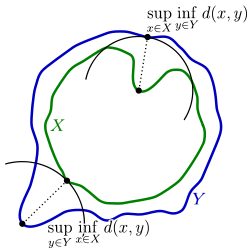
\includegraphics[scale=0.8]{images/hausdorff_distance.png} }
    \caption{Hausdorff distance in $\R^2$}
\end{figure}

In the absence of an analytic expression for the Hausdorff distance in our case,
we attempt to compute it using Monte Carlo methods with the following procedure.
\begin{itemize}\nospace
    \item Fix $n$, let $k$ vary.
    \item Sample from the parameter space $\R^{nk + n + k}$.
    \item Transform under $f: \R^{nk + n + k} \to M_n^k$.
    \item Compute Hausdorff distances between the images under $f$.
    \item Use these distances to approximate $d_H(M_n^k, M_n^{k+1})$.
\end{itemize}
Using intuition from low-dimensional $\R^n$, it seems at least plausible that
this procedure should give a good estimate.  If the finite samplings are
$\epsilon$-dense subsets of the spaces, the error should be on the order of
$\epsilon$.  One way to check to see if the sampling is sufficiently dense is to
sample twice from the same subspace; the Hausdorff distance should be close to
zero.  Furthermore, because there is an exponential dependence on the
parameters, it should be sufficient to sample the parameter space near the
origin.

This procedure was carried out, first in a Python implementation, and then in a
C++ implementation for better performance.  Parts of the parametrization can be
formulated in terms of matrix operations; the C++ version used the linear
algebra library \texttt{armadillo}, which is backed by the \texttt{BLAS} (Basic
Linear Algebra Subprograms) library, implemented in Fortran.  The performance
difference is approximately a factor of 100.

The source is currently hosted under version control at
\mbox{\texttt{https://github.com/apribadi/thesis-code}}.

\section{February 6, 2012}

There are two items on the agenda:
\begin{enumerate}
    \item Instead of sampling randomly from the parameter space, take a lattice
    from the parameter space.
    \item Instead of computing the Hausdorff distance from two random samples,
    and a quadratic algorithm in the number of samples, sample from the `outer'
    distribution, and find the proper inner one using gradient descent.
\end{enumerate}

The first task was implemented.  As before, code is at
\mbox{\texttt{https://github.com/apribadi/thesis-code}}.  Unfortunately, this
does not do much to alleviate the curse of dimensionality.  The number of
samples is still exponential in the number of parameters.  The degenerate case
of a lattice is the hypercube
\[
    \{ (x_1, \ldots, x_{nk+n+k}) \mid x_i \in \{-1, 1\}\} \subset \R^{nk+n+k}.
\]
Here, of course, we are sampling $2^{nk+n+k}$ points.  For a decent run of
values of $k$ (enough to pick up patterns), we want $n=2$.  (The $n=1$ case is
trivial; we get the whole space immediately.)

For the second task, you can download libraries to do the training for you.  I
tried the \texttt{Shark} machine learning library at
\mbox{\texttt{http://image.diku.dk/shark/sphinx\_pages/build/html/index.html}}.
I was not, however, able to get it to work.  (A note for future passers-by:
Perhaps a third of the time actually implementing things was spent arguing with
the C++ compiler and linker.  This is unfortunate.)

\sout{
There is, however, another significant problem.  Going back the non-lattice case
(as would have been approached using these ML libraries), there isn't actually a
non-trivial bound on distances!  Specifically, with notation as before,}
\[
    d_H(M_n^{k_1}, M_n^{k_2}) = 1
\]\sout{
for any $k_1$, $k_2$, where the Hausdorff distance is derived from the total
variation distance.  This is because with only the binary independence model, we
can get arbitrarily close to a $\delta$-function, i.e., for $\epsilon > 0$, we
have $p_v \in \Delta$ such that}
\begin{align*}
    p_v[X = v] &= (1 - \epsilon)^N \\
    p_v[X \ne v] &\le \epsilon
\end{align*}
\sout{ for any $v$.  Then for $v \ne u$,}
\[
    d(p_v, p_u) \ge (1 - \epsilon)^N - \epsilon \to 1
\]
\sout{
as $\epsilon \to 0$.  The maximal total variation distance \ldots.}

The above \sout{struck out} thoughts don't actually invalidate this approach,
though they \emph{do} make it impossible to compute a bound via the naive
method suggested in the midyear report, bounding the distance of a step from any
starting point (where we use the total variation distance -- the hope was to use
something more suitable).

Results for the hypercube mapping are
\begin{verbatim}
    Hausdorff distance between k=0 and k=1 is: 0.310871
    Hausdorff distance between k=1 and k=2 is: 0.346856
    Hausdorff distance between k=2 and k=3 is: 0.210349
    Hausdorff distance between k=3 and k=4 is: 0.171509
    Hausdorff distance between k=4 and k=5 is: 0.101923
\end{verbatim}
and the program does not compute any further values.  This is a downward trend,
as one would expect.
    

\section{February 13, 2012}

We're going to talk about symmetry groups of graphical models.  

\subsection{A digression into hierarchical log-linear models}
We first take
another look at graphical models, following \cite{DSS09}

Specifically, we work with undirected graphs and binary-valued nodes.  We can
formulate undirected graphical models in terms of a hierarchical log-linear
model.

\begin{definition}
    Let $V$ be a finite set.  A \emph{simplicial complex} is a collection
    $\Gamma \subset \ps(V)$ of subsets of $V$ such that $F \in \Gamma$ and $S
    \subset F$ implies that $S \in \Gamma$.  
\end{definition}
The elements of $\Gamma$ are called \emph{faces} of $\Gamma$ and the
inclusion-maximal faces are the \emph{facets} of $\Gamma$.  Notice that to
describe a simplicial complex it is sufficient to list only its facets.

With notation as in section 1.2 of \cite{DSS09}, we have the following
definition.

\begin{definition}
    Let $\Gamma \subset \ps(V)$ be a simplicial complex.  For each facet $F$, we
    introduce $2^{|F|}$ positive parameters $\theta_{i_F}^{(F)}$.  The
    associated \emph{hierarchical log-linear model} is
    \[
        \ms_\Gamma = \cdel*{p \in \Delta_{2^{|V|} - 1}
            \mid p_i = \frac{1}{Z(\theta)} \prod_{F} \theta_{i_f}^{(F)}
        }
    \]
    where $Z(\theta)$ is the appropriate normalizing constant.
\end{definition}

For every hierarchical log-linear model, there exists a matrix $A$ with integer
entries for which
\[
    \ms_\Gamma = \ms_A = \cdel*{
        p \in \Delta \mid \log p \in \mathrm{rowspan}(A)
    }
\]
and we can therefore find an associated Markov basis.

Via the Hammersley-Clifford theorem, a graphical model is a hierarchical
log-linear model where the facets correspond to the maximal cliques.
Equivalently, a subset of the nodes of the graph is in the simplicial complex if
and only if the subgraph on those nodes is a complete graph.
Because we're interested in Boltzmann machines, we are actually interested in a
slightly different model.

\begin{definition}
    A \emph{binary graph model} of a graph $G = (V, E)$ is the hierarchical log-linear
    model associated with the simplicial complex
    \[
        \Gamma = \{\{v\}\mid v \in V\} \cup \{ \{v, w\} \mid (v, w) \in E\}
    \]
\end{definition}
If there are no cliques of size three or more (say, if the graph is bipartite), then
the notion of a binary graph model corresponds with that of a usual undirected
graphical model.

\subsection{Symmetries of graphical models}
Say that we have a graphical mode, and that it has $m$ nodes, all binary valued.
Either a usual undirected graphical model or a binary graph model will do.

There are $N = 2^m$ states, indexed by binary strings, e.g. $(0, 0, 1, 0,
\ldots, 1)$.  A probability distribution is a function on the binary strings
\[
    p: \{0, 1\}^m \to \R
    \qquad
    p(x) > 0
    \qquad
    \sum_{x \in \{0, 1\}^m} p(x) = 1
\]
and can naturally be embedded in $\R^N$ where basis vectors are associated
with states.

Let $\ms \subset \Delta \subset \R^N$ be the associated model.  Let $G = S_2
\wr H$ be the wreath product of $S_2$ and $H$, where $H$ is the automorphism
group of the graph.  Recall that an automorphism of a graph is a permutation of
its nodes such that edges are preserved.  There is a natural action of $G$ on
the set of states.  Essentially, $H$ acts on the nodes of the graph, and each
copy of $S_2$ permutes a binary state.  Write this action $g(x)$ for $g \in
G$.

This group action induces an action on $\R^N$
\[
    g(p)(x) = p(\inv g x)
    \qquad
    \text{for $p \in \R^N$}
\]
which is in fact a permutation representation of $G$.  Additionally, it seems
clear that $g(\ms) = \ms$ for all $g \in G$, i.e. that the model is invariant
under the action of the wreath product group.  A proof would merely involve
carefully stating the relevant ideas.

\subsection{Star graphs}
We're going to be looking at the simplified case of a RBM with only one hidden
node.  First, look at the model before marginalization.  The associated graph is
a star graph.
\begin{figure}[H]
    \centering
    \scalebox{1}{ 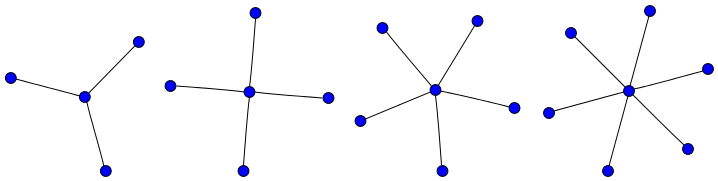
\includegraphics[scale=0.5]{images/star_graphs.png} }
    \caption{Some star graphs}
\end{figure}
Let $n$ be the number of leaf nodes.  Assume that $n \ge 2$.  The automorphism
group of the graph is $2^n$ (acting on $n+1$ nodes); any of the leaves can be
permuted but the central node must be fixed.

\subsection{Invariant Subspaces}

Given a linear group action on $\R^N$, it is natural to consider subspaces of
$\R^N$ invariant under the action, and especially irreducible subspaces.

We first ignore graph automorphisms, and only consider binary swaps `internal'
to nodes.  Then we have the group $J = (S_2)^m$ acting on the states.  The
representation theory of $J$ is easy, of course, because it is abelian.

Fix some state $s_0$ (the choice is arbitrary).  The group $J$ acts transitively
on states, and is in fact regular.  We can write every state uniquely as
$g(s_0)$ for $g \in J$.  Thus the action of $J$ on $\R^N$ corresponds to the
regular representation of $J$.

Let $J$ have generators $J = \adel*{g_1, \ldots, g_m}$,
all of order 2.  To every bit vector $b = (b_1, \ldots, b_m) \in \{0, 1\}$ there
corresponds the irreducible representation
\[
    \rho_b((g_1)^{c_1 }\cdots (g_m)^{c_m}) = (-1)^{b_1 c_1} \cdots (-1)^{b_m c_m}
\]
For $m=2$, the character table looks like
\[
\begin{matrix}
    & 1 & g_1 & g_2 & g_1g_2 \\
    \chi_1 & 1 & 1 & 1 & 1 \\
    \chi_2 & 1 & -1 & 1 & -1 \\
    \chi_3 & 1 & 1 & -1 & -1 \\
    \chi_4 & 1 & -1 & -1 & 1 \\
\end{matrix}
\]
Then, a decomposition of $\R^N$ (for $m=2$) into irreducible invariant spaces is
\[
    \R^4 = 
    \adel*{\begin{bmatrix}1 \\ 1 \\ 1 \\ 1\end{bmatrix}}
    \oplus
    \adel*{\begin{bmatrix}1 \\ -1 \\ 1 \\ -1\end{bmatrix}}
    \oplus
    \adel*{\begin{bmatrix}1 \\ 1 \\ -1 \\ -1\end{bmatrix}}
    \oplus
    \adel*{\begin{bmatrix}1 \\ -1 \\ -1 \\ 1\end{bmatrix}}
\]
and similarly for greater $m$.

For any vector $v \in \R^N$, we can project $v$ into these subspaces.  The
appropriate inner product is, I think,
\[
    \adel*{v, w} = \frac 1 {N} \sum_i v_i w_i
\]
so that it matches the inner product for the regular representation of
$(S_2)^m$, and the subspaces are orthogonal.  In any case, since the
irreducibles are 1-dimensional, we can take basis vectors from the irreducibles
and consider their coefficients in a decomposition.

Consider probability distributions $p \in \R^N$ (i.e. $\sum p_i = 1$, $p_i \ge
0$), decomposed into these invariant subspaces.   The coefficient of the trivial
representation will always be $\tfrac 1 N$, because the other vectors all sum to
zero.  This is because (considering the permutation action) the identity has $N$
fixed points, and all other group elements have no fixed points.  The sums
hold because these are permutation characters.

The projection of the uniform distribution is
\[
    \mathrm{uniform} = (\tfrac 1 N, 0, \ldots, 0)
\]
and the delta distributions look like
\[
    (0, \ldots, 0, 1, 0, \ldots, 0)
    = \tfrac 1 N (\epsilon(1), \ldots, \epsilon(N))
\]
where $\epsilon(i)$ is \ldots something.

We can move from the group $J = (S_2)^m$ to $G = S_2 \wr H$ where $H$ is, again, the
automorphism group of the graph.  The invariant subspaces of $G$ are composed of
those of $J$, grouped together, as $J$ is a subgroup of $G$.

\subsection{Log-linearity}

There is a bit of a mismatch between the model $\ms \subset \Delta \subset \R^N$
and $\R^N$ as a representation.  Specifically, if $p, q \in \ms$ then for $\mu,
\lambda \in \R$, the subspace $\adel{\mu p + \lambda q}$ may not intersect $\ms$.

If that were the case, then we would be looking at arbitrary mixtures of the
model.  We have seen, however, that arbitrary mixtures of the independence model
produces the trivial model, i.e. the whole simplex $\Delta$.

Notice the form of a (hierarchical) log-linear model.
\[
    \ms_\Gamma = \ms_A = \cdel*{
        p \in \Delta \mid \log p \in \mathrm{rowspan}(A)
    }
\]
Here, $\log p$, rather than $p$, lies within a linear subspace.  Because the
logarithm is component-wise, everything about permutation representations still
hold.  So perhaps we should consider $\log p$ in relation to invariant
subspaces.

\section{February 20, 2012}

Tentative outline of thesis:
\lspace

\noindent Statistical models
\begin{itemize}\nospace
\item geometry (simplex)
\item hypothesis testing
\item maximum-likelihood fitting
\item inference
\end{itemize}

\noindent Log-Linear models
\begin{itemize}\nospace
\item graphical
\item hierarchical
\item general
\end{itemize}

\noindent Bases of an integer lattice
\begin{itemize}\nospace
\item Markov basis
\item Lattice ideal $M_A = \adel{p^{b^+} - p^{b^-} \mid b \in B}$
\end{itemize}

\noindent Algorithms
\begin{itemize}\nospace
\item MCMC sampling from fiber $F(u)$ with Markov basis
\item Birch's theorem
\end{itemize}

\noindent Symmetries, groups and representations
\begin{itemize}\nospace
\item representations of $S_2 \wr S_n$
\end{itemize}

\noindent Binary models with $S_2 \wr S_n$ symmetry.
\begin{itemize}\nospace
\item classification?
\end{itemize}


\begin{thebibliography}{100}
    \bibitem[BCR98]{BCR98} Bochnak, Coste, Roy.  Real Algebraic Geometry.  1998.
    \bibitem[Ben09]{Ben09} Bengio.  Learning Deep Architectures for AI. 2009.
    \bibitem[CLO98]{CLO98} Cox, Little, O'Shea.  Using Algebraic Geometry.  1998.
    \bibitem[CLS09]{CLS09} Cox, Little, Schenck.  Toric Varieties.  2009.
    \bibitem[CMS09]{CMS09} Cueto, Morton, Sturmfels. Geometry of the Restricted Boltzmann Machine.  2009.
    \bibitem[Cos09]{Cos09} Michel Coste.  An Introduction to Semialgebraic Geometry.  2002.
    \bibitem[CTY10]{CTY10} Cueto, Tobis, Yu.  An Implicitization Challenge for Binary Factor Analysis. 
    2010.
    \bibitem[DS98]{DS98} Diaconis and Sturmfels.  Algebraic Algorithms for Sampling
    from Conditional Distributions. 1998.
    \bibitem[DSS09]{DSS09} Drton, Sturmfels, Sullivant. Lectures on Algebraic
    Statistics. 2009.
    \bibitem[GMS06]{GMS06} Geiger, Meed, Sturmfels.  On the Toric Algebra of Graphical Models. 2006.
    \bibitem[Hin07]{Hin07} Hinton.  A Fast Algorithm for Deep Belief Nets.  2007.
    \bibitem[MA10]{MA10} Montufar, Ay.  Refinements of Universal Approximation
    Results for Deep Belief Networks and Restricted Boltzmann Machines.  2010.
    \bibitem[Mon10]{Mon10} Montufar.  Mixture Models and Representational Power of
    RBM's, DBN's and DBM's.  2010.
    \bibitem[PS03]{PS03} Pachter, Sturmfels.  Tropical Geometry of Statistical Models. 2003.
    \bibitem[Ric09]{Ric09} Riccomagno.  A Short History of Algebraic Statistics.  2009.
    \bibitem[Top02]{Top02} Topics in Algebraic Geometry and Geometric Modeling:
    Workshop on Algebraic Geometry and Geometric Modeling July 29 -- August 2,
    2002 (Contemporary Mathematics).  Ed. by Goldman and Krasauskas.

    \bibitem[Wat09]{Wat09} Watanabe.  Algebraic Geometry and Statistical Learning Theory.  2009.

    \bibitem{A4} Garcia, Stillman, Sturmfels.  Algebraic Geometry of Bayesian Networks.  2003.
    \bibitem{A6} Pachter, Sturmfels.  Algebraic Statistics for Computational Biology.  2005.

    \bibitem{B1} Domingos, Poon. Sum-Product Networks: A New Deep Architecture. 2011.
    \bibitem{B2} Smith, Zwiernik.  The Geometry of Independence Tree Models with Hidden Variables.
\end{thebibliography}


\end{document}
